\documentclass[sigconf]{acmart}

\sloppy
\settopmatter{printacmref=false} % Removes citation information below abstract
\renewcommand\footnotetextcopyrightpermission[1]{} % removes footnote with conference information in first column
\pagestyle{plain} % removes running headers
\usepackage{booktabs} % For formal tables
\usepackage{caption}
\usepackage{subcaption}
\usepackage{indentfirst}
\usepackage{graphicx}
% Rights management information. 
% This information is sent to you when you complete the rights form.
% These commands have SAMPLE values in them; it is your responsibility as an author to replace
% the commands and values with those provided to you when you complete the rights form.
%
% These commands are for a PROCEEDINGS abstract or paper.
% \copyrightyear{2018}
% \acmYear{2018}
% \setcopyright{acmlicensed}
% \acmConference[Woodstock '18]{Woodstock '18: ACM Symposium on Neural Gaze Detection}{June 03--05, 2018}{Woodstock, NY}
% \acmBooktitle{Woodstock '18: ACM Symposium on Neural Gaze Detection, June 03--05, 2018, Woodstock, NY}
% \acmPrice{15.00}
% \acmDOI{10.1145/1122445.1122456}
% \acmISBN{978-1-4503-9999-9/18/06}

%
% These commands are for a JOURNAL article.
%\setcopyright{acmcopyright}
%\acmJournal{TOG}
%\acmYear{2018}\acmVolume{37}\acmNumber{4}\acmArticle{111}\acmMonth{8}
%\acmDOI{10.1145/1122445.1122456}

%
% Submission ID. 
% Use this when submitting an article to a sponsored event. You'll receive a unique submission ID from the organizers
% of the event, and this ID should be used as the parameter to this command.
%\acmSubmissionID{123-A56-BU3}

%
% The majority of ACM publications use numbered citations and references. If you are preparing content for an event
% sponsored by ACM SIGGRAPH, you must use the "author year" style of citations and references. Uncommenting
% the next command will enable that style.
%\citestyle{acmauthoryear}

%
% end of the preamble, start of the body of the document source.
\begin{document}

%
% The "title" command has an optional parameter, allowing the author to define a "short title" to be used in page headers.
\title{Comparative Study of Multi-Label Classification Techniques for Movie Genre Classification Based on Plot Overview}

%
% The "author" command and its associated commands are used to define the authors and their affiliations.
% Of note is the shared affiliation of the first two authors, and the "authornote" and "authornotemark" commands
% used to denote shared contribution to the research.
\author{Matt McCreesh}
\email{mmccrees@stevens.edu}
\affiliation{%
\institution{Stevens Institute of Technology}
	\city{Hoboken}
	\state{New Jersey}
}

\author{Kaitlynn Prescott}
\email{kprescot@stevens.edu}
\affiliation{%
	\institution{Stevens Institute of Technology}
	\city{Hoboken}
	\state{New Jersey}
}

% By default, the full list of authors will be used in the page headers. Often, this list is too long, and will overlap
% other information printed in the page headers. This command allows the author to define a more concise list
% of authors' names for this purpose.
\renewcommand{\shortauthors}{Trovato and Tobin, et al.}
\linebreak\linebreak
%

\begin{abstract}
\noindent We compared multiple machine learning algorithms for the task of genre classification of movies based on the plot overview. We use a large dataset of movies and apply techniques such as Logistic Regression, k-Nearest Neighbors, Convolutional Neural Networks, and Long Short Term Memory Recurrent Neural Networks. We implement these models using multi-label classification, and test on a 20 genre dataset and a smaller 6 genre dataset. Our models display promising results, with our larger dataset, the total correct predictions across all labels is more accurate, however on the smaller dataset, our per label prediction was more accurate.
\end{abstract}

\keywords{text classification, multilabel classification, neural networks, RNN, LSTM, CNN, Logistic Regression, Nearest Neighbors}

%
% This command processes the author and affiliation and title information and builds
% the first part of the formatted document.
\maketitle

\section{Introduction}
For our final project, we implemented, evaluated, and compared several machine learning classification algorithms for predicting the genre of a movie based on textual overviews of the movie.  This was a supervised, multi-label classification problem.

This is an important problem for use in marketing and movie recommendations on streaming platforms. If a streaming service can accurately predict the genre of new movies that are entering their service, they can classify them for viewers who want to see movies of a specific genre. This allows them to predict and provide more fine-grained genres than the movie might come labelled as. It also can give the benefit from a marketing perspective of ensuring that the released plot overview of a movie matches the genre it is aimed for, as a drama that has a description that comes off comedic may need to have changes to the released plot overview to better market the movie.

Some potential applications of this include learning the correlation between movie descriptions and movie genres to help categorize movies on streaming services.  Often, the only data a person or company has about a movie, other than the entire movie itself, is a short paragraph long overview of what the movie is.  With movies becoming such a dominating force in the entertainment industry, a tool like this can be extremely helpful to moviegoers and potential filmmakers alike.

Our project is in scope for this class as we used several supervised learning classification techniques covered in this course. Techniques include including: logistic regression, k-Nearest Neighbors, a single hidden layer neural network, two convolutional neural network, a simple recurrent neural network, LSTM, and bidirectional LSTM for classification.  We wrote. We use tf-idf and word2vec to get the text in a useable form for our algorithms and neural networks. We also wrote our own implementation for multi label accuracy metrics to evaluate and compare our approaches.  We used cross validation to get the best results from all classification techniques used. 


\section{Background and Related Work}

Classifying movie genres is not a new problem. One approach to movie genre classification was in a paper titled ``Characterization of Movie Genre Based On Music Score'' [3] which also appeared in the IEEE database.  This research involved classifying movie genres based on non-vocal music from films.  They used Support Vector Machines to do both pairwise and multiclass genre classification considering genres of romance, horror, drama, and action.  One drawback of this is that it requires access to music scores from movies which is not always available and is not available in our dataset for this study.  In other previous work titled ``Movie Genre Classification with Convolutional Neural Networks'' [2], video of movie trailers was used to classify the genre of the movie using a convolutional neural networks. A limitation of this approach is that it requires access to many movie trailers.  Storage can become an issue if downloading trailer video of movies in bulk. As our data is different, we took a different approach than the approaches described in these papers. 

One paper more applicable for our project is ``Movie Genre Classification from Plot Summaries using Bidirectional LSTM'' [1]. This paper that appeared in the 2018 12th IEEE International Conference on Semantic Computing which discussed using Long Short Term Memory, a recurrent neural network, to classify movie genres based on the movie's plot summary.  They describe considering the genre information represented by each sentence using Bi-LSTM. They also took a document level approach analyzing summaries as a whole with the LSTM approach.  They compared this to using standard RNNs (recurrent neural networks) at a sentence and document level.  Lastly, they compared this to a logistic regression model using bag of words and TD-IDF. In this research, movies were classified by genres of thriller, horror, comedy, and drama. Using the sentence level Bi-LSTM approach, precision, accuracy, macro f1, and micro f1 score were all between .67 and .68. A drawback of the paper is that it only classified movies with coarse grained genres and it was multi-class but not mult-label.  In our research try to predict more fine-grained genres and perform multilabel classification.  We do, however, incorporate document level LSTM and document level Bidirectional LSTM in our research.


\section{Approach}
In our project, we are attempting to implement several classification techniques using known techniques, apply those models for the multi-label movie genre from overview problem, and compare them in terms of several classification metrics. There are two basic techniques to multi-label classification: problem transformation and algorithm adaptation. Problem transformation involves separating a multi-label problem into multiple single-label problems, while algorithm adaptation involves adapting a single-label classification algorithm to perform multi-label classification [springer citation]. We mostly chose to implement problem transformation.

Algorithms we aim to compare include: K-Nearest Neighbors, Logistic Regression, a standard hidden single layer Neural Network fed data from an embeddings layer, a Convolutional Neural Network, a simple Recurrent Neural Network, LSTM, and Bidirectional LSTM. K-Nearest-Neighbors (KNN), is a non-parametric method used for single label classification that can be be extended to multi-label classification problems. Logistic Regression is a linear classifier that can be used for the multi-class case by doing binary classification for each label. The other approaches involve neural networks and allow for non-linear decision boundaries and can solve complicated problems. They can take a long time to train but once trained prediction can be fast and with high accuracy performance.They can be extended to the multi-label problem by making them classify each output as an independent binary problem with the sigmoid activation function and binary cross-entropy loss function.  

Our goal is to compare the above approaches, some of which we have studied in class for single label classification problems, and compare their results for multi-label classification. Instead of proposing a new approach, our goal is to compare the performance of existing approaches when used to do multi-label classification of movie genres based on paragraph long overviews of the movie. In terms of efficiency, we compare them in terms of time to train, time to predict. In terms of evaluation metrics, we compare their accuracy, precision, recall in both the binary single label sense as well as the multi-label sense. We also define hamming loss, the percent of all possible labels that are incorrectly classified, and report its additive inverse, the percent of all possible labels correctly classified. 

\section{Experimental Design}
\subsection{Languages and Tools}
Our project was written in Python 3 in Jupyter notebook files.  Each group of similar experiments was done in one file.  We used several publicly available packages and tools.  Some of these include gensim, scikit-learn (sklearn), pandas, numpy, nltk, and Keras with the TensorFlow backend. 

\subsection{Data}
The dataset we used came from the Kaggle Box Office Prediction competition, but instead of predicting box office revenue we will predicted genre.  The dataset has 3000 examples in it, each of a unique movie.  The dataset includes recent movies as well as movies dating back to the 1930s. The dataset can be found at https://www.kaggle.com/c/tmdb-box-office-prediction/data.

The data set includes many potentially useful pieces of information about a movie. There are 23 columns including the target field. The target field we used for predictions is the genre category, which was originally a feature that could have been used predict revenue. In this category, each row is a json object containing, as strings, the genres associated with that movie. Our main training field was the plot overview. In this category, each row contains a string, usually three to four sentences, of the given overview of the movie. The remaining fields, including the title, director, cast, release year, and revenue were ignored, as they are not useful for text classification. Given our goal is to compare classification techniques, and some of those techniques (LSTM, for example) are based off of sequential data, it would be unfair to include other features in this comparison study. Although the tagline and keyword fields could be useful, we focused on the plot overview for testing our algorithms. This constrained us to a very specific goal: use movie overviews to predict genres of movies and compare results using several methodologies. A future direction would be to build classifiers that take in other features and build an ensemble classifier to predict genres of movies. 

There are a few important things to note about our dataset.  There are 20 genre labels that appear throughout the data set, and any movie can be assigned any number of these labels.  These labels do not come with percentages of how much a movie belongs to that genres, and the order of genres does not indicate how strongly a movie is an example of that genre relative to other genres listed.  These genres in the dataset are: War, Family, Science Fiction, Thriller, Horror, Romance, Drama, Foreign, Documentary, Fantasy, Western, History, Comedy, Action, Adventure, Animation, Crime, Music, TV Movie, and Mystery. The dataset is also somewhat unbalanced, both in terms of binary classification looking at one feature at a time as well as in terms of the multilabel aspect where some labels were much more common than other labels.  Some genres, such as Drama, were very common.  Other genres, such as Foreign, were significantly less common. For several genres, over ninety percent of movies were not labelled as being of that genre. This meant that accuracy for predicting some of the labels could be very high even if the prediction algorithm for that label was to just always predict false.  Our evaluation metrics of single label binar precision and recall capture this problem, and our focus on multi-label definitions of accuracy, precision, and recall also help us get a better idea of how our models perform in this unbalanced scenario. 

One more problem with the data is that genre was not the intended target field.  For this reason, we found that many movies that should have been classified as several of the genres were only listed as belonging to a few of the categories.  Some movies that were listed as more specific categories should have been listed as drama but were not. Other movies were only listed as being a drama or a comedy, but in reality could have been labelled as other genres as well.  This meant that our ground truth was not perfect because of limitations of the data we worked with. 

To handle unbalanced datasets, subsampling is often used for single label prediction.  In [1], they randomly subsampled equal numbers of movies for each genre they were trying to classify.  However, while that approach would work for the multiclass problem, it may not work as well for the multi-label problem, as even after subsampling each class will likely be unbalanced with less examples with each label than without. One approach to this was to manually combine labels in to coarser grained labels.  We ran all of our models once using all of using the labels as given, and another time using coarser grained, manually mapped labels. 

\begin{figure}
	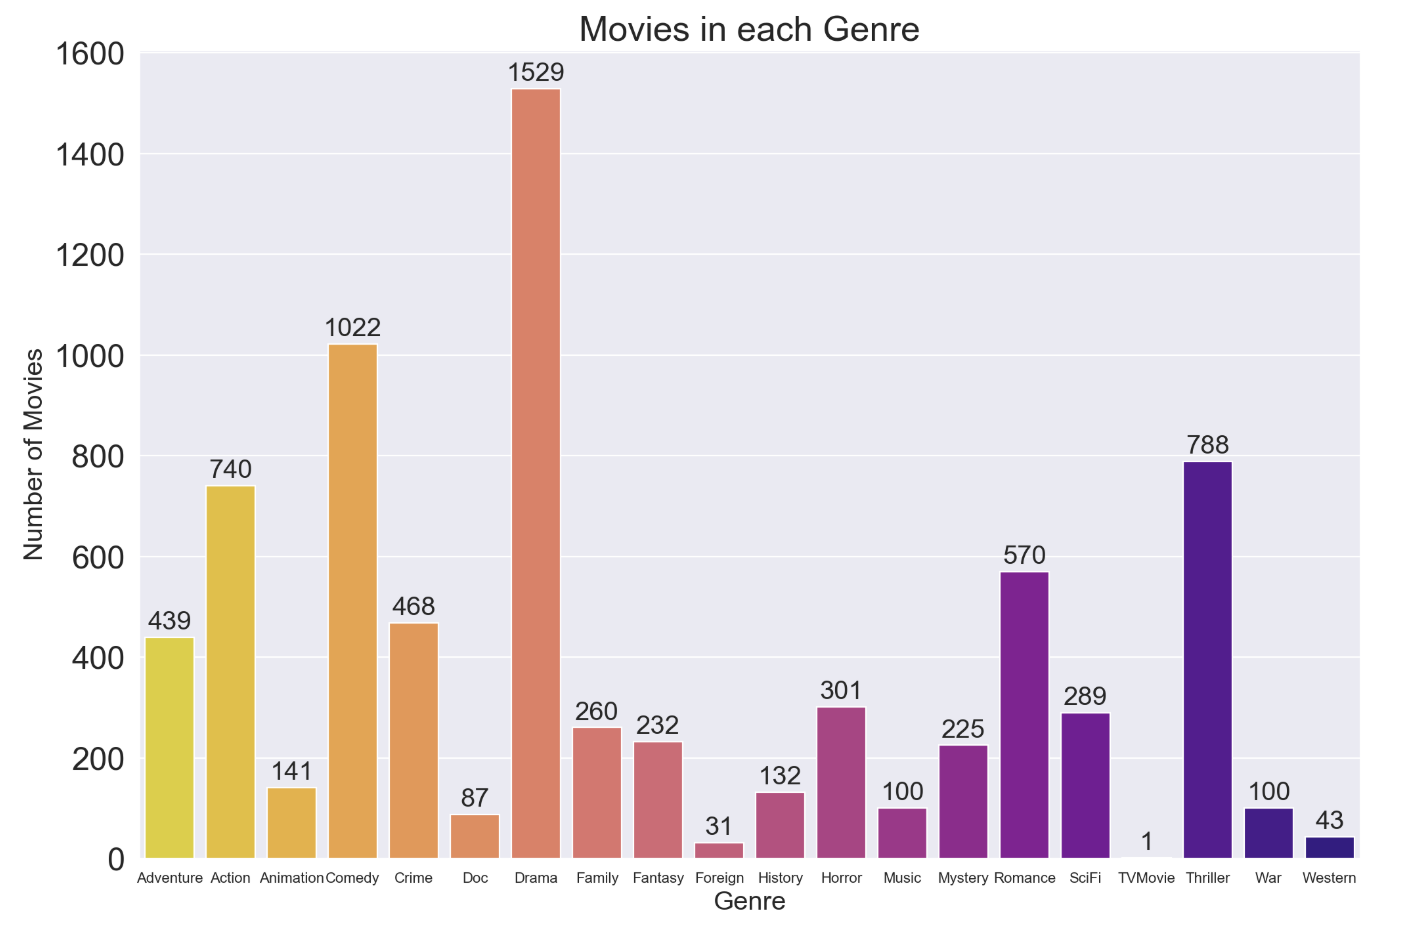
\includegraphics[width=\linewidth]{all_genres.png}
	\caption{All Genres}
	\label{fig:all}
\end{figure}


\subsection{Data Preprocessing}
Before implementing any of our learning algorithms, we first needed to do feature extraction and clean our data set.  We used pandas to read in the csv data of our dataset.  We then removed rows that did not have the overview field or did not have any genres associated with it.  This did not eliminate too many rows, but it gave us data that was better to work with.

We then needed to get data in a form that would be ideal to work with for each classifier we used.  Because the data we were interested in was textual, and our algorithms didn't directly deal with text. We first cleaned up the text we were working with.  We filtered out all characters besides letters, numbers, and spaces. As movie overviews were only a few sentences, we chose to work with them in whole instead of breaking down to a sentence level. Therefore, removing periods was not a problem.  We kept numbers in the text when cleaning the text, hoping to find if common numbers were useful for classifying certain genres, though this may not have helped classification much.  As we are solving a classification problem as opposed to trying to build a language model, we found that removing stopwords was a good idea. We used the nltk library to remove stopwords. Once text was cleaned, we needed to represent it in a better format. 

For logistic regression and kNN, we chose to use tf-idf to get text into a vector format. Tf-idf was a good choice for logistic regression and kNN as both algorithms works with feature vectors. 
Tf-idf is term frequency -- inverse document frequency.  It gives weights for each word occurring in an overview by taking into account how often the word appears in the overview and how often it appears in other overviews. We originally planned on using a bag of words for both logistic regression and kNN, but preliminary research into text classification pointed us in the direction of tf-idf being a better approach for our problem.  A future direction could be to use more advanced approaches, such as doc2vec, to get a vector for each movie overview.  
For our deep learning and neural network models, we wanted to work with sequences of text.  We used word2vec to get word embeddings for each word in our training data.

For our neural networks and deep learning approaches, we used word embeddings as features.  Each word was represented by a word vector that was learned at the embedding layer of the neural network.  We first tokenized our training text. We then passed in the tokenized training words to word2vec to get 32 bit vectors for each word and store them in a 100,000 row matrix for the most common 100,000 words.  We then used Keras's Sequences to convert words in our data to integers indexing the matrix used by word2vec.  For each cleaned overview, we produced a sequence of 150 of those integers, padding with 0s if the text had less than 150 words. These sequences would be fed to each neural network architecture we made, with every architecture starting with an embeddings layer that stored the original matrix for word2vec and was trainable to improve the embeddings. 

The last part of data preprocessing was splitting our data between training and testing.  In every experiment, we got a random train-test split where 20 percent of the data was used for testing and the remaining 80 percent was used for training. 

\begin{figure}
	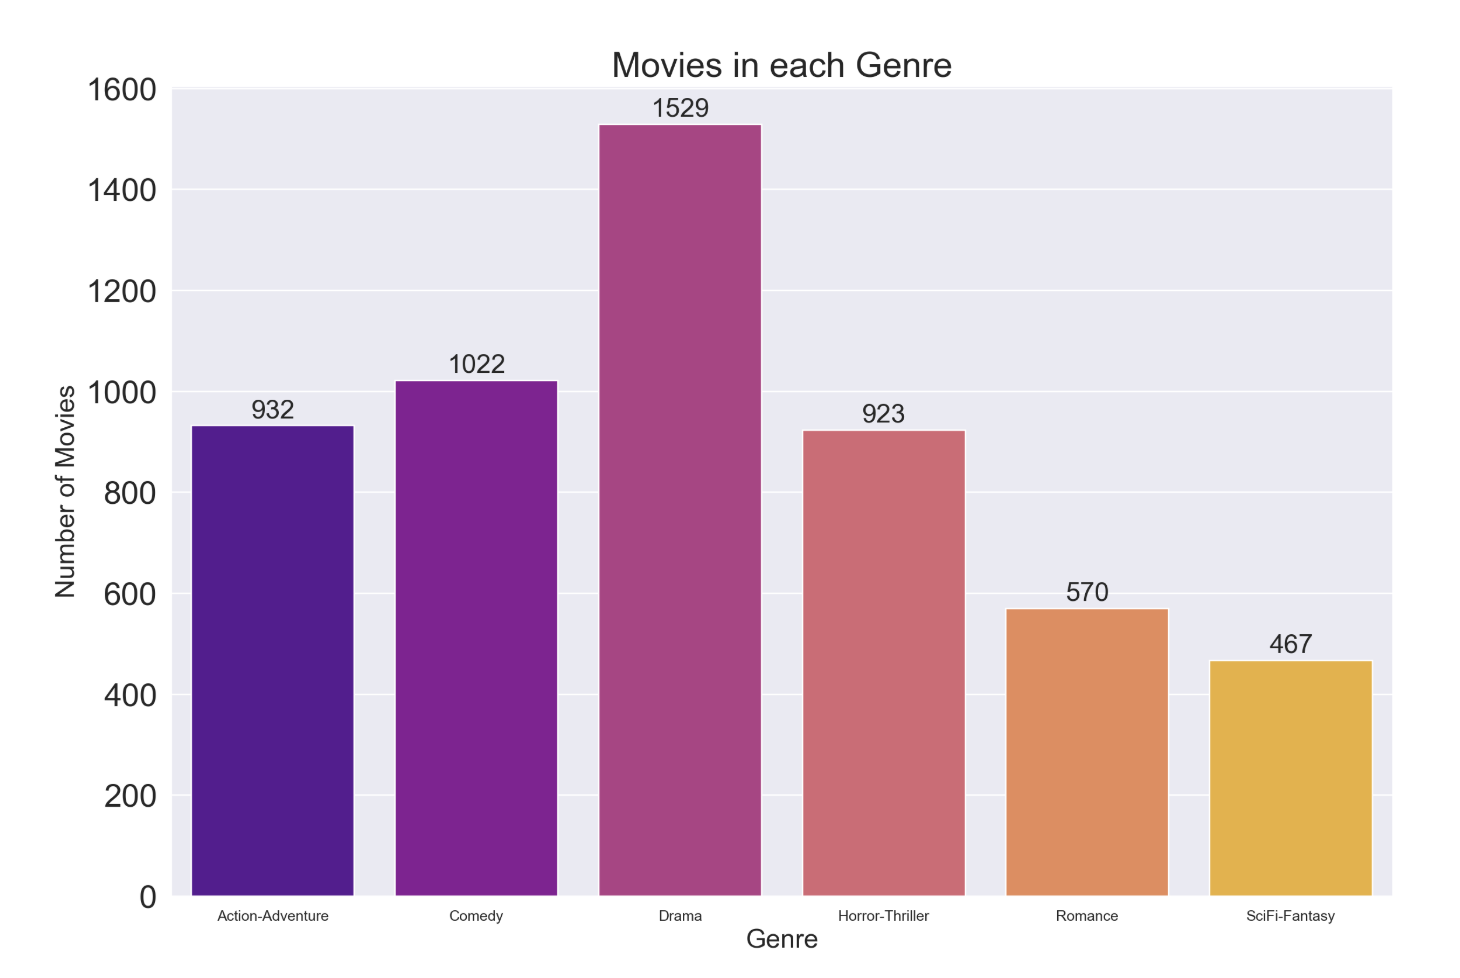
\includegraphics[width=\linewidth]{reduced_genres.png}
	\caption{Less Genres}
	\label{fig:less}
\end{figure}

\subsection{Logistic Regression}
We included Logistic Regression in order to have a parameterized linear classifier in our study. With logistic regression, we used the approach of transforming the multi-label problem to single-label classification problems for each label. We used scikit-learn's Pipeline, OneVsRestClassifier, and TfidfVectorizer to build a binary, single label model for each label.  To do this, we wrote a class (which we called MulitLabelLogisticRegression) that created a pipeline for label and stored the pipeline in a dictionary that mapped label names to its pipeline. In the pipeline, first was the TfidfVectorizer which would fit the tf-idf vector on the training data and then produce a td-idf vector on testing data during testing.  Next in the pipeline was a OneVsRestClassifier which used sklearn's LogisticRegression classifier with the liblinear solver to do binary classification. 

When an instance of our MultiLabelLogisticRegression class was created, a dictionary of label to label vector indices was passed in.  The MultiLabelLogisticRegression would create a pipeline for each label in the dictionary and store those in a dictionary mapping labels to pipelines. The class then offered a fit method, a predict method, and a predictThreshold method. To do multilabel classification, fit would take in an array of strings (the overviews of the training data) and the corresponding label matrix and do training to allow for finding td-idf vectors for future textual inputs as well as converting the training data to td-idf vectors. Fit also converted the training data text to td-idf form and trained each labels logistic regression classifier on each of those vectors. Predict would take in an array of textual input, run the prediction function of each label's classifier, and combine the results into a labels vector.  PreidctThreshold would do the same thing except it would also take in a threshold and do predict proba with. It would set a label to 1 if the probability of being 1 was over the threshold and set it to 0 in the other case. 

The reason we defined a predictThreshold function was to handle the unbalanced dataset by changing the decision threshold to be something other than .5.  As this was a multilabel problem, subsampling as done in [1] would likely still produce unbalanced binary sets for each label.  Therefore, we instead did k cross validation to find the optimal threshold which was shown as a good way to get better predictions for logistic regression in [citation]. We did k fold cross validations with different threshold values, found the result that gave the highest multi-label accuracy, and used that as the threshold value.  It should be noted that we probably could have gotten better results by independently finding each optimal threshold for each category, but in order to simplify the interface to our classifier and keep the cross validation short we left that for future work. 

\subsection{kNN}
The technique we used for k-Nearest neighbors was the adapted algorithm approach. We started with using the MLkNN algorithm from the python library skmultilearn. This algorithm implements multi-label classification derived from k-Nearest Neighbors. Rather than simply picking a k value that may be suitable, we augmented the algorithm using cross validation. By repeating the cross validation on various k values using cross val score, we are able to pick the appropriate k value that will return the highest accuracy. The k value with the highest cross validation score was used for the training and testing in the multi-label k-NN classification. 

Single Hidden Layer Neural Network:
Another technique we attempted for multi-label classification was using a single hidden layer neural network, where the single hidden layer was given input from an embeddings layer. We used Keras, with the TensorFlow backend, to build the neural network.  The architecture of the neural network was an embeddings layer that was given a matrix of pre-trained word vectors from gensim's word2vec.  We allowed the embeddings layer to be trainable so it could learn word-embeddings on the fly from our initial embeddings. The embeddings layer took in sequences of indices into the passed in embeddings matrix and these sequences were padded. The output from the embeddings layer was then flattened to a vector so it could be used as input into our single hidden layer network. It should be noted that the embedding layer could probably have been replaced with a different input layer that just took in the sequences and did not deal with embeddings, as the embeddings would just be immediately flattened anyway.  However, we felt that including the embeddings layer and them flattening would give a good baseline for other architectures we used that relied on word embeddings.  The hidden layer had 256 hidden units which used ReLu as the activation function.  Lastly, there was an output layer.  The output layer had as many units as there were labels being predicted. As the data came with 20 possible labels, this meant if we tried to classify every label we would have 20 units here.  These units used the sigmoid activation function. In the multi-class problem, generally softmax is used as the output layer activation function, but we are doing multi-label classification, so sigmoid is used to do binary classification on each label.  The loss function used, for the same reason, is binary cross-entropy. 

\subsection{Convolutional Neural Network}
To build the Convolutional Neural Network (CNN), we started with a convolutional layer, Conv1D, which is ideal for text classification. We then added a pooling layer, GlobalMaxPooling1D, to avoid flattening the data. Then we added a Dense layer with the rectified linear unit (relu) activation function, a Dropout layer to help avoid overfitting, and a Dense layer using the sigmoid activation function. Finally, we compile the model with the binary cross entropy loss function and the Adam optimizer. We also implemented a CNN with multiple filter sizes to allow discovering features about two words, three words, and four words together. 

\subsection{Recurrent Neural Network (RNN)}
A Recurrent Neural Network allows the network to continue learning at each step, and work over sequences of data. We chose to add Keras's SimpleRNN layer to implement the RNN. We included the two Dense layers, and compiled with the binary cross entropy loss function and Adam optimizer.

\subsection{Long Short Term Memory (LSTM)}
The base of LSTM is a recurrent neural network. To build it, we use the LSTM layer, with a dropout parameter of 0.25 to prevent overfitting. We then included two Dense layers, a hidden layer and the output layer, and we compiled with the binary cross entropy loss function, and the Adam optimizer.

\subsection{Bidirectional-LSTM (Bi-LSTM)}
To implement the Bidirectional LSTM layer, we add a Bidirectional layer in Keras, passing in the LSTM layer as its input to it's constructor. This can help improve the model by running LSTM on both the as-is input sequence and a reversed copy of the input sequence. We add the two Dense layers and compile with the binary cross entropy function and the Adam optimizer.

\section{Experimental Results}
\subsection{Logistic Regression}
The results of logistic regression on all labels displayed an accuracy for each label between 54 percent and 100 percent. For the multi-label part of our model, the accuracy was approximately 40 percent, the precision was approximately 57 percent, and the recall approximately 54 percent. Overall, the total percentage of correctly decided labels was 88 percent. For the reduced label set, the accuracy was between 65 percent and 88 percent. For the multi-label problem, the accuracy was approximately 54 percent, the precision was approximately 62 percent, and the recall approximately 75 percent. Overall, the percentage of correctly decided labels was 75 percent.

\subsection{k-Nearest Neighbors}
The results from the multi-label kNN on all labels displayed an accuracy of approximately one percent, a precision of approximately seven percent, and a recall of approximately four percent. The results from the multi-label kNN on the reduced labels displayed an accuracy of approximately 14 percent, a precision of approximately 50 percent, and a recall of about 29 percent. It is, again, evident that reducing the number of possible genres will increase the accuracy. However, while the metrics are much better with a reduced number of metrics, there is still room for improvement. Because we used the built in function for this problem, we could not define accuracy metrics for each individual metric, we only had the accuracy metrics across all labels.

\subsection{Neural Network}
The results from the standard neural network on all labels displayed an accuracy between 60 percent and 100 percent, however some of the better accuracies are only better because there were zero predictions made for rare labels. For the multi-label problem, the accuracy was approximately 23 percent, the precision approximately 59 percent, and the recall approximately 26 percent. In total, the percentage of labels that were correctly decided was 88 percent. The results on the reduced labels displayed an accuracy between 57 percent and 89 percent. For the multi-label problem, the accuracy was approximately 24 percent, the precision 53 percent, and the recall 27 percent. The percentage of the total labels correctly labeled was about 70 percent.

\subsection{Convolutional Neural Network}
The results from the convolutional neural network on all labels displayed an accuracy for each label between 54 percent and 100 percent, however some of the better accuracies are only better because there were zero predictions. For the multi-label problem, the accuracy was approximately 23 percent, the precision was approximately 45 percent, and the recall was approximately 28 percent. The total percentage of labels decided correctly is 86 percent. For the reduced label problem, the accuracy for each label was between 61 percent and 89 percent. For the multi-label problem, the accuracy was approximately 36 percent, the precision was approximately 57 percent, and the recall was approximately 44 percent. The total amount of labels decided correctly is 72 percent.

We also ran a CNN with multiple filter sizes so we do not filter on the same groups of words at a time. With this model on all labels, the accuracy for each label was between 59 percent and 100 percent. For the multi-label problem, the accuracy was approximately 25 percent, the precision was approximately 52 percent, and the recall was approximately 30 percent. In total, about 87 percent of the labels were correctly decided. On the reduced label problem, the accuracy on each label was between 61 percent and 88 percent. For the multi-label problem, the accuracy was approximately 36 percent, the precision was 55 percent, and the recall 42 percent. In total, the amount of labels correctly decided was about 70 percent. 

\subsection{Recurrent Neural Network}
The results for the recurrent neural network displayed an accuracy for each label was between 53 percent and 100 percent. For the multi-label problem, the accuracy was approximately 21 percent, the precision 42 percent, and the recall 27 percent. The total percentage of labels correctly decided was 85 percent. For the recurrent network on the reduced label problem, the accuracy for each label was between 52 percent and 90 percent. For the multi-label problem, the accuracy was approximately 22 percent, the precision was 38 percent, and the recall 27 percent. In total, the percentage of correctly decided labels was about 63 percent.

\subsection{Long Short Term Memory}
For all labels, the accuracy for each label of LSTM was between 57 percent and 100 percent. For the multi-label problem, the accuracy was approximately 29 percent, the precision was approximately 48 percent, and the recall was approximately 38 percent. In total, the percentage of of labels that were correctly decided was 86 percent. On the reduced label problem, the accuracy for each label was between 62 percent and 87 percent. On the multi-label problem, the accuracy was approximately 48 percent, the precision was approximately 68 percent, and the recall was approximately 64 percent. The percentage of correctly decided labels was approximately 72 percent.

\subsection{Bidirectional-LSTM}
Finally, for Bi-LSTM, the accuracy of each label was between 56 percent and 100 percent. For the multi-label problem, the accuracy was approximately 27 percent, the precision was approximately 50 percent, and the recall was approximately 34 percent. Overall, the percentage of correctly decided labels was around 86 percent. As for the reduced labels, the accuracy of each label was between 63 percent and 88 percent. For the multi-label problem, the accuracy was approximately 50 percent, the precision 59, and the recall 70 percent. In total, the percentage of all labels correctly decided was about 73 percent.

\section{Analysis of Results}
Of all the methods we used, LSTM and Bi-LSTM were the best at correctly predicting the labels of the reduced label set, however it was the basic neural net and the CNN which had the best accuracy on predicting the labels of the full set. This is interesting, because LSTM is designed for text classification, but it was outperformed on the full set of labels. This may just be a result of a dataset where the ground truth for some rare labels was not exact.  It was also interesting to notice that the RNN model was the least successful at predicting the labels correctly by about seven percent. 

Out of all our models, the absolute best scenario was the basic neural network model on the full set of labels. It is intriguing that this is the case because every layer we added to the base neural net is theoretically supposed to create a more accurate model. It is also interesting that the logistic regression model outperformed every neural network in both the full label set and the reduced label set when the threshold for classification was adjusted, when neural networks should have been better at predicting labels as it is likely a non-linear function that would need to be predicted.

\section{Conclusion}
In this paper, we have implemented and analyzed several techniques to do text classification of paragraph long movie overviews to classify movies based on genre. This was a multi-label text classification problem, and we had some approaches to modified the problem into multiple single label problems, while another approach was to modify algorithms to work for multilabel approaches. We used the non-parametric approach of k-Nearest-Neighbors and used an implementation of the algorithm modified to do multi-label prediction. The k-Nearest-Neighbors algorithm worked on text data represented in tf-idf vector format. In addition to this method, we used Logistic Regression on tf-idf vectors representing text.  Logistic regression is a linear classifier and did not perform very well right away.  However, when we used k-fold cross validation to choose a classification threshold that optimized multi-label accuracy, Logistic Regression had competitive performance on multi-label metrics compared to more advanced classifiers. 

The more advanced classifiers included simple neural networks as well as some deep learning approaches. We used a single hidden layer neural network, where the hidden layer sat behind an embeddings layer that could learn word embeddings.  We compared this to two Convolutional Neural Network architectures, a simple Recurrent Neural Network, a neural network with an LSTM layer, and a Neural Network with a Bi-Directional LSTM layer. Ultimately, we found that our approach using LSTM and our threshold-modified Logistic Regression gave us the highest accuracy for predicting genres from overviews. We also narrowed our genre possibilities to fewer genres and noticed improved performance of all techniques, but similar relative results as when solving the unmodified label prediction problem. 

We implemented single label classification metrics (precision, accuracy, and recall on a per label basis), as well as multi-label accuracy, precision, and recall metrics. We compared each approach in terms of these metrics, as well as in terms of time to train or predict. 
There were many challenges we've discussed, including not entirely accurate ground-truth, unbalanced data, and limited information that could be conveyed about genre by short overviews that don't go into detail about the plot. Ultimately, we believe that a larger dataset, a dataset with better ground truth, and a dataset with entire plot summaries instead of short overviews may be useful for improving our accuracy and getting better results. A major issue was that our classifiers could get high accuracy on some genres by never classifying any movie as that genre, as some genres were quite rare. 

\section{Future Work}
It is fairly evident that a classifier that only takes in the overview as input may not be the best classifier. To make a stronger and more accurate classifier, the classifier should be able to take in more input, such as numerical data (i.e. revenue, runtime, and popularity) and json objects (i.e. keywords, cast and crew, and production companies). 

In order to do this, one could implement a Stacked Generalization model, which uses a classifier that combines a pool of base classifiers to reduce generalization error. This would allow the classifier to use the first stage predictions as features. One could also use a Blending classifier, which removes a portion of the training dataset as a holdout on which the stacker trains. This would have less information leaks compared to the stacker, but may be susceptible to overfitting. Either of these methods would work with both linear and non-linear models, making it diverse and a strong classifier. One could also use Bagging, creating random samples of the data, building a classifier for each sample, and combining the results. Boosting provides sequential learning on the predictions by first training on the full dataset, and the following predictors will learn on data based on the results of the previous one. The major benefits of Ensembling are a stronger, more stable model and a more accurate model, however there are still dangers of overfitting the training data. While we did not implement an Ensemble model, any of these methods would be able to provide a more stable model, and would be able to use all of the given data to provide a more accurate model.

\section{References}

[1] A. M. Ertugrul and P. Karagoz, ``Movie Genre Classification from Plot Summaries Using Bidirectional LSTM,'' 2018 IEEE 12th International Conference on Semantic Computing (ICSC), Laguna Hills, CA, 2018, pp. 248-251.

\noindent[2] G. S. Simões, J. Wehrmann, R. C. Barros and D. D. Ruiz, ``Movie genre classification with Convolutional Neural Networks,'' 2016 International Joint Conference on Neural Networks (IJCNN), Vancouver, BC, 2016, pp. 259-266.

\noindent[3] A. Austin, E. Moore, U. Gupta and P. Chordia, ``Characterization of movie genre based on music score,'' 2010 IEEE International Conference on Acoustics, Speech and Signal Processing, Dallas, TX, 2010, pp. 421-424.


\end{document}
